\documentclass[11pt,a4paper]{article}
\usepackage[hyperref]{acl2018}
\usepackage{times}
\usepackage{latexsym}
\usepackage{graphicx}
\usepackage{url}

\aclfinalcopy

\title{Transfer Learning for Abstractive Text Summarization with Pointer-Generator Networks}

\author{Rutika Banakar \\
 School of Information, University of California, Berkeley \\
 {\tt rutikasb@berkeley.edu} \\}
 
\date{July 23, 2018}

\begin{document}
\maketitle
\begin{abstract}
  In this work, we model abstractive text summarization with hybrid pointer-generator networks on the CNN/Daily Mail dataset and transfer the learnings to New York Times Annotated Corpus. The idea of transfer learning is to use knowledge learnt from one task or domain to apply to a new task or domain instead of starting from the scratch. Through this work, we attempt to study the transfer of learnings from neural networks trained over CNN/DailyMail dataset to the NYT corpus.
\end{abstract}

\section{Introduction}

Summarization is an important challenge of natural language understanding. The aim is to produce a condensed representation of an input text that captures the core meaning of the original. Most successful summarization systems utilize extractive approaches that crop out and stitch together portions of the text to produce a condensed version. In contrast, abstractive summarization attempts to produce a bottom-up summary, aspects of which may not appear as part of the original.

Transfer Learning uses the knowledge learnt by solving a problem pertaining to one task or domain (source) and apply it to a different task or domain (target). In the field of computer vision for example, models are rarely trained from scratch and features extracted from a state-of-the-art CNN pre-trained on ImageNet is used to train a new model. Similarly, we could use weights learned from a model trained over one corpus and fine tune it with a different corpus.

In this work, we train a pointer-generator network on CNN/Daily Mail corpus and then transfer the knowledge to NYT corpus. Although both the corpora are from same domain i.e., new articles, the NYT corpus contains articles for restaurant reviews, book review, opinion articles, interview articles and other varied articles. Hence the transfer of learning is not entirely trivial. And it will also help to avoid over-fitting to the CNN/Daily Mail data.

\section{Related Work}
 
\subsection{Pointer-Generator Networks}
\citep{Rush2015} were the first to apply abstractive text summarization on DUC 2004 and Gigaword datasets using feed-forward neural language model. Their approach was further improved upon with recurrent neural networks \citep{Chopra2016}, abstract meaning representations \citep{Takase2016}, hierarchical networks \citep{Nallapati2017}. \citep{Nallapati2016} used Attention Encoder-Decoder RNNs and showed that they achieve state-of-the-art performance on the Gigaword and DUC corpora. They also released a new CNN/Daily Mail dataset with very long source documents and multi-sentence summaries, and established performance benchmarks on this dataset for further research. The same authors used hierarchical RNNs \citep{Nallapati2017} and found that it significantly outperformed their previous model in terms of the ROUGE metric.

\citep{See2017} used a hybrid between sequence-to-sequence attention model which is similar to the model proposed in \citep{Nallapati2016} and a pointer network \citep{Vinyals2015} on the CNN/Daily Mail dataset and showed that it out performed the benchmarks set by \citep{Nallapati2016} by at least 2 ROUGE points.

\subsection{CNN/Daily Mail Corpus}

\citep{Hermann2015} created two datasets using news articles for Q\&A research. The datasets contain 90k and 197k documents. \citep{Nallapati2016} modified these datasets for the task of text summarization. The original authors used the human generated abstractive summary bullets from new stories in \textit{CNN} and \textit{Daily Mail} websites as questions and the news stories as the corresponding passages. They also released the scripts to crawl and extract pairs of passages and questions from these websites. With a simple modification to this script \citep{Nallapati2016} were able to convert the summary bullets of each article into a multi-sentence text summary. The corpus has 286,817 training pairs, 13,368
validation pairs and 11,487 test pairs.

\subsection{New York Times Annotated Corpus}

\citep{NYT} released the New York Times Annotated corpus which contains 1.8 million New York Times articles. The dataset is aimed to encourage research in leveraging background information about entities (entity salience). The dataset however, also contains about 600,000 articles with hand written summaries.

\section{Methods}

\begin{figure*}
  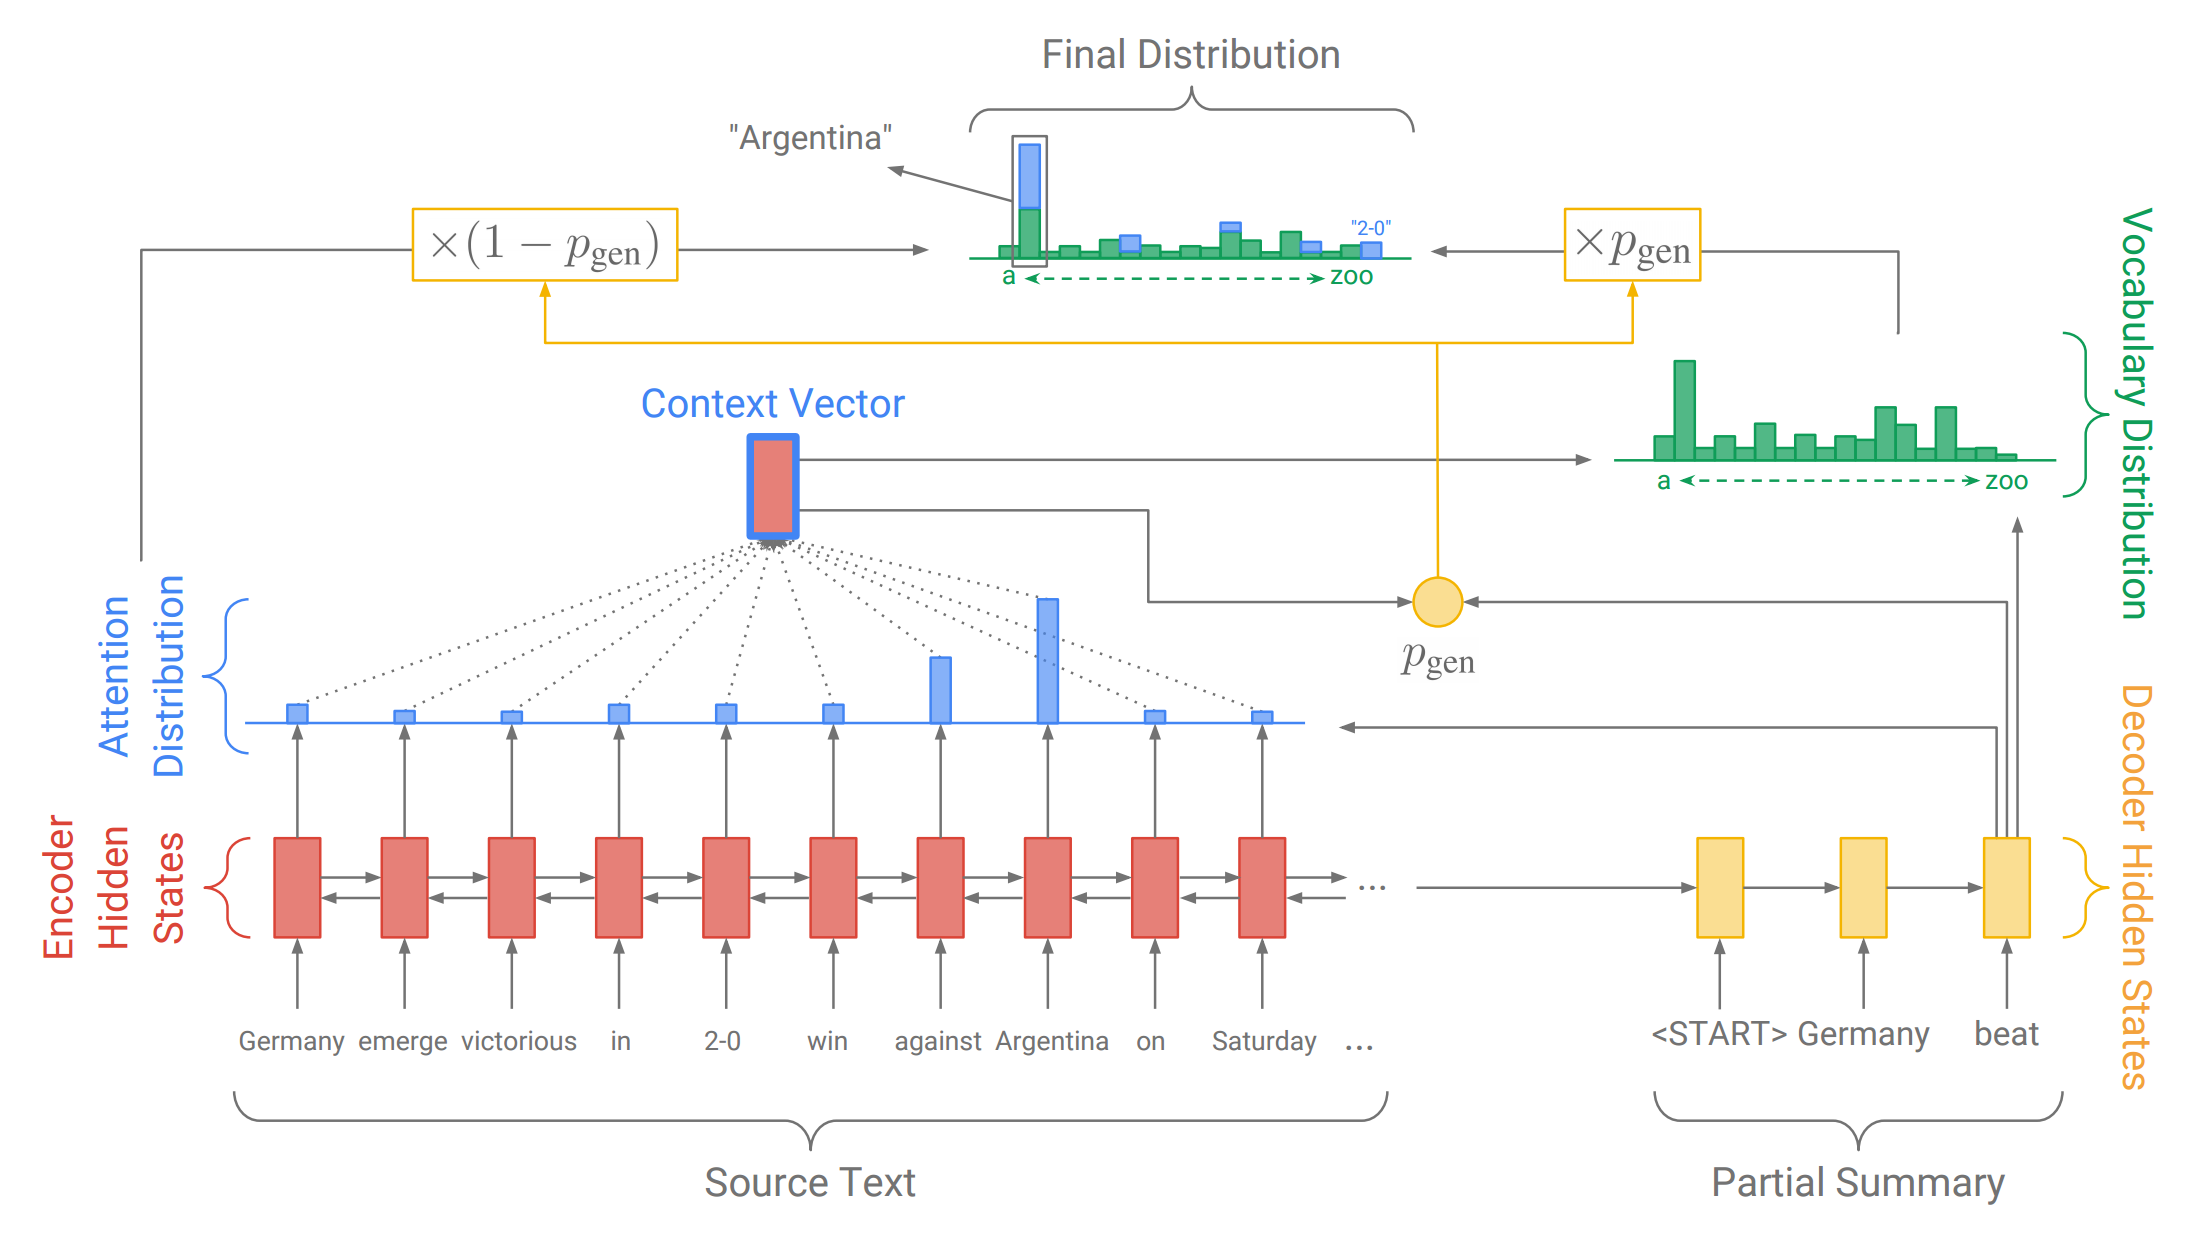
\includegraphics[width=\textwidth,height=8cm]{pointer-gen.png}
  \caption{Pointer-generator model \citep{See2017}}
  \label{fig:pointer-gen}
\end{figure*}

The pointer-generator is a hybrid network that can choose to copy words from the source via pointing, while retaining the ability to generate words from the fixed vocabulary. This model makes it easy to copy words from the source text and even copy out-of-vocabulary words from the source text.

We first train a pointer-gen network on CNN/Daily Mail dataset, which will be our source task/domain, resulting in a \textit{source model}. We'll then perform a number of transfer experiments with varying number of article-summary pairs from NYT corpus which is our target task/domain.

\section{Results}

\section*{Acknowledgments}

\bibliographystyle{acl_natbib}
\bibliography{textsummary}

\end{document}
